% E-Voting Machine © 2024 by S4Y Solutions is licensed under CC BY-NC-ND 4.0.
% To view a copy of this license, visit https://creativecommons.org/licenses/by-nc-nd/4.0/
%
% v3: aligned with the design docs (docs/) and the working demo. Same look as v1.
% Build: pdflatex pitch-deck-v3.tex  (needs texlive-latex-extra and texlive-pictures)
\documentclass[11pt,aspectratio=169]{beamer}

% ****************
% ***** INFO *****
% ****************
\usepackage[english]{babel}
\title{e-Voting Machine}
\subtitle{Investor Presentation}
\author[Sergey Dolin]{Sergey Dolin \\
\href{mailto:sergey@s4y.solutions}{\scriptsize{sergey@s4y.solutions}}}
\institute{S4Y Solutions}
\newcommand{\currentyear}{\the\year}
\date{\currentyear}

\definecolor{main}{HTML}{0000FF}
\definecolor{ok}{HTML}{1D7A46}
\definecolor{bad}{HTML}{B3261E}
\definecolor{warn}{HTML}{9A6700}
\setbeamercolor{structure}{fg=main}

\newcommand{\copyrightnote}{
    \vfill
    \begin{flushleft}
    \tiny
    E-Voting Machine \textcopyright~\currentyear~by S4Y Solutions is licensed under
    \href{https://creativecommons.org/licenses/by-nc-nd/4.0}{CC BY-NC-ND 4.0.}
    \end{flushleft}
}

% *****************
% ***** THEME *****
% *****************
\usetheme{Luebeck}
\usepackage{helvet}
\renewcommand{\familydefault}{\sfdefault}
\setbeamertemplate{footline}{}
\setbeamertemplate{navigation symbols}{}

\usepackage{tikz}
\usetikzlibrary{arrows.meta,positioning}
\usepackage{booktabs}
\usepackage{array}
\newcolumntype{L}[1]{>{\raggedright\arraybackslash}p{#1}}
\newcolumntype{B}[1]{>{\raggedright\arraybackslash\bfseries}p{#1}}
\usepackage{xcolor}

\tikzset{
    box/.style={draw, rounded corners=3pt, fill=blue!8, align=center, font=\scriptsize, minimum height=2.2em, text width=5.2em},
    pub/.style={box, fill=green!10},
    arr/.style={-{Stealth[length=2mm]}, thick},
    lbl/.style={font=\tiny, align=center}
}
\newcommand{\yes}{\textcolor{ok}{\ding{51}}}
\usepackage{pifont}
\newcommand{\trusted}{\textcolor{warn}{trusted}}

% ********************
% ***** DOCUMENT *****
% ********************
\begin{document}

% ***** Title *****
\begin{frame}{}
    \vspace{\fill}
    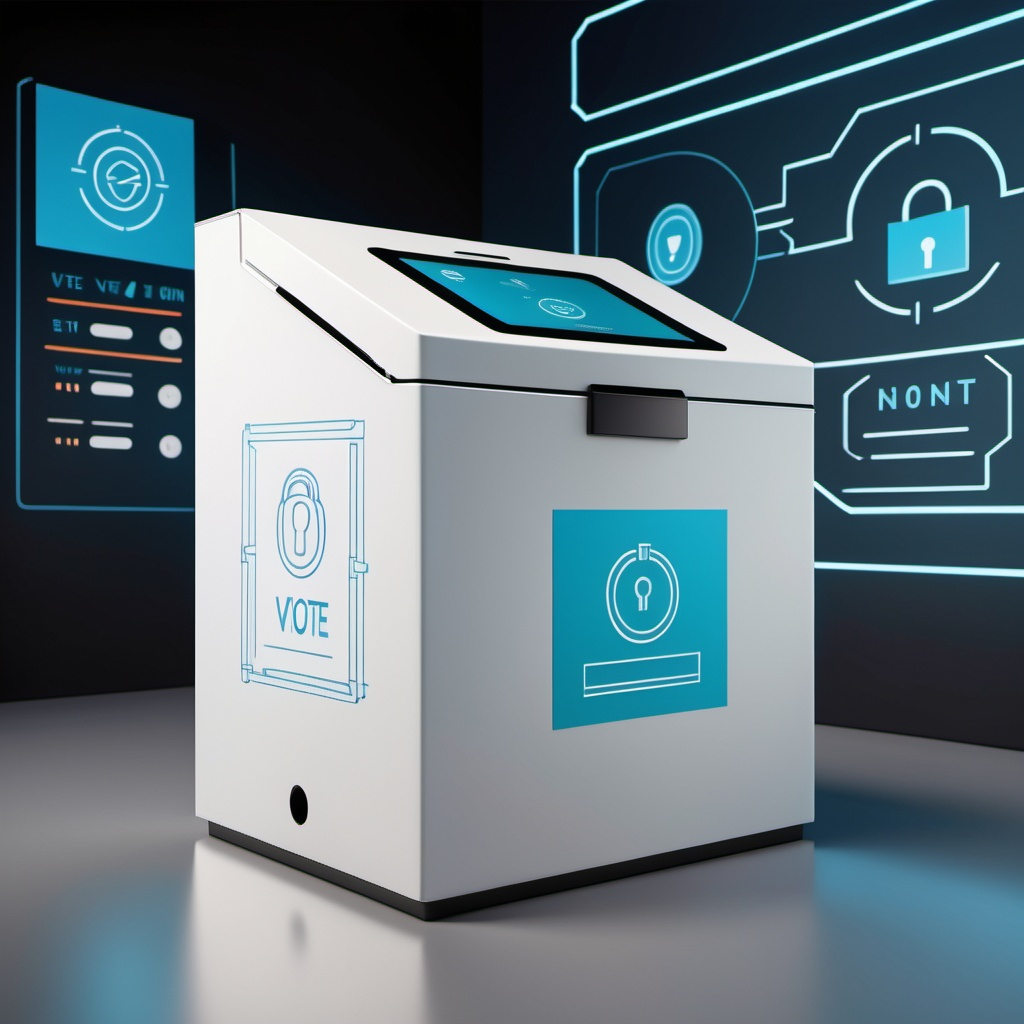
\includegraphics[width=0.12\linewidth]{voting-machine}
    \vspace{\fill}

    \Large\color{main}\inserttitle

    \medskip
    \large\color{black}\insertsubtitle

    \vspace{\fill}
    \footnotesize\insertinstitute

    \vspace{\fill}
    \textbf{Author:} \insertauthor

    \medskip
    \insertdate
    \copyrightnote
\end{frame}

% ***** Problem *****
\begin{frame}{The challenges of voting online}
    \begin{itemize}
        \item \textbf{Verifiable and secret at once.} A voter wants proof that their vote counted;
        a secret ballot means nobody may learn how they voted.
        \item \textbf{No voting booth.} At home, a voter can be watched, pressured or paid
        to vote a certain way, and asked to show proof.
        \item \textbf{Identity.} Each eligible voter must get exactly one say, with
        a predictable level of certainty about who they are.
    \end{itemize}

    \medskip
    \begin{block}{Published work has tackled this for twenty years}
        Estonia's i-voting, Helios, JCJ/Civitas and MACI each solve part of it, at the cost of
        complex cryptography that is hard to explain to the people who vote.
    \end{block}
    \copyrightnote
\end{frame}

% ***** Idea *****
\begin{frame}{The idea: revocable votes on a public, add-only ledger}
    \begin{exampleblock}{Change your vote at any time while the voting is open}
        A voter can cancel their vote and vote again. Every vote is a public \texttt{+1};
        a cancellation is a public \texttt{-1} that is \textbf{not linked} to the vote it cancels.
    \end{exampleblock}

    \begin{columns}[T]
        \column{0.5\textwidth}
        \begin{block}{For the voter}
            A receipt finds their vote on the public ledger, so they can check it was counted as cast.
        \end{block}
        \column{0.5\textwidth}
        \begin{alertblock}{Against a coercer}
            The receipt proves the vote was cast, not that it still counts. The voter can change
            it later, alone, and the coercer cannot tell.
        \end{alertblock}
    \end{columns}

    \medskip
    \small The tally is the sum of the ledger: anyone can add it up.
    \copyrightnote
\end{frame}

% ***** Flow *****
\begin{frame}{How it works}
    \centering
    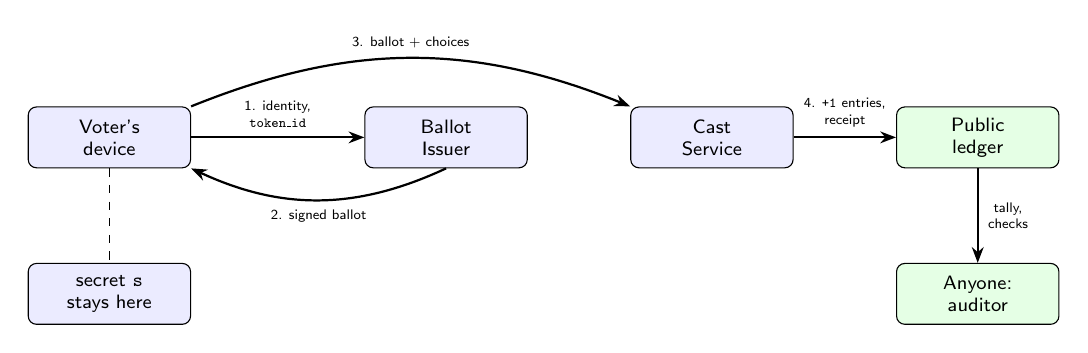
\begin{tikzpicture}[node distance=6mm and 13mm]
        \node[box] (voter) {Voter's\\device};
        \node[box, right=22mm of voter] (issuer) {Ballot\\Issuer};
        \node[box, right=of issuer] (cast) {Cast\\Service};
        \node[pub, right=of cast] (ledger) {Public\\ledger};
        \node[pub, below=12mm of ledger] (audit) {Anyone:\\auditor};
        \node[box, below=12mm of voter] (secret) {secret \texttt{s}\\stays here};

        \draw[arr] (voter) -- node[lbl, above] {1. identity,\\\texttt{token\_id}} (issuer);
        \draw[arr] (issuer.south) to[bend left=25] node[lbl, below] {2. signed ballot} (voter.south east);
        \draw[arr] (voter.north east) to[bend left=22] node[lbl, above] {3. ballot + choices} (cast.north west);
        \draw[arr] (cast) -- node[lbl, above] {4. \texttt{+1} entries,\\receipt} (ledger);
        \draw[arr] (ledger) -- node[lbl, right] {tally,\\checks} (audit);
        \draw[dashed] (voter) -- (secret);
    \end{tikzpicture}

    \vspace{2mm}
    \begin{itemize}\small
        \item \texttt{token\_id = H("token"\,\textbar\,s)}, receipt \texttt{= H("cast"\,\textbar\,s)}: both derived from a secret only the voter holds.
        \item \textbf{Re-vote:} the voter proves the old vote with \texttt{s}; the ledger gets \texttt{-1} entries with no receipt, and the voter a new ballot.
        \item Every entry is signed and chained to the previous one by its hash: nothing can be rewritten unnoticed.
    \end{itemize}
    \copyrightnote
\end{frame}

% ***** Terms *****
\begin{frame}{The building blocks}
    \small
    \renewcommand{\arraystretch}{1.25}
    \begin{tabular}{B{0.22\textwidth}L{0.7\textwidth}}
        \toprule
        Ballot token & Signed by the Issuer. One first ballot per eligible voter; a re-vote ballot only in exchange for a cancelled vote \\
        Receipt & The cast ID. Finds the voter's \texttt{+1} entries on the ledger \\
        Add-only ledger & \texttt{+1} and \texttt{-1} entries, signed by the operator and hash-chained. Nothing is ever edited or deleted \\
        Voter registry & Public: random pseudonyms and whether each one received a ballot. Never who they are \\
        ``Smart contract'' & The published, deterministic rule that checks and applies each entry. No blockchain is required \\
        Readable signatures & Every signed value is shown as plain text plus its real signature tag, so a tampered line visibly fails \\
        \bottomrule
    \end{tabular}
    \copyrightnote
\end{frame}

% ***** Checks *****
\begin{frame}{What anyone can check}
    \small
    \renewcommand{\arraystretch}{1.2}
    \begin{tabular}{L{0.62\textwidth}ccc}
        \toprule
        & \textbf{Voter} & \textbf{Anyone} & \textbf{Operator} \\
        \midrule
        My vote was recorded as I chose & \yes & & \\
        The tally equals the sum of the ledger & \yes & \yes & \\
        The ledger was not rewritten (signatures, hash chain) & \yes & \yes & \\
        No more net votes than ballots issued & \yes & \yes & \\
        Nobody took a ballot in my name & \yes & & \\
        \midrule
        Every cancellation was made by the vote's owner & & & \trusted \\
        The issuer does not link my identity to my ballot & & & \trusted \\
        \bottomrule
    \end{tabular}

    \medskip
    \footnotesize The last two rows are the honest limits of the first version. The roadmap removes them.
    \copyrightnote
\end{frame}

% ***** Cheat *****
\begin{frame}{Try to cheat: live in the demo}
    Each attempt runs against the real system and is rejected with its reason:
    \begin{itemize}
        \item Ask for a second ballot \hfill \textcolor{ok}{rejected: already issued}
        \item Cast the same ballot twice \hfill \textcolor{ok}{rejected: token already spent}
        \item Forge the issuer's signature on a ballot \hfill \textcolor{ok}{rejected: not signed by the issuer}
        \item Cancel someone else's vote without its secret \hfill \textcolor{ok}{rejected: no matching vote}
        \item Cancel the same vote twice \hfill \textcolor{ok}{rejected: already cancelled}
        \item Edit a ledger line \hfill \textcolor{ok}{its signature turns red}
    \end{itemize}
    \medskip
    After every attempt, the public auditor re-runs its checks and they all still pass.
    \copyrightnote
\end{frame}

% ***** Prior art *****
\begin{frame}{Where this stands among existing systems}
    \footnotesize
    \renewcommand{\arraystretch}{1.2}
    \begin{tabular}{B{0.15\textwidth}L{0.37\textwidth}L{0.38\textwidth}}
        \toprule
        System & Against coercion & Difference \\
        \midrule
        Estonia i-voting & Re-voting; the last vote counts & Encrypted votes; earlier ones are dropped at tally time \\
        Helios, Belenios & None: a voter can prove their vote & Encryption and trustees; hard to explain \\
        JCJ, Civitas & Fake credentials & Strongest model; heavy tally, hard to use \\
        MACI & Re-voting and key changes & Encrypted messages, proofs of a correct tally \\
        \textcolor{main}{This project} & \textcolor{main}{Re-voting inside the ledger} & \textcolor{main}{Public \texttt{±1} entries: a tally anyone can add up} \\
        \bottomrule
    \end{tabular}

    \medskip
    \small
    \textbf{Stand-out:} explainability, re-voting without a separate tally step, an honest staged trust
    model, and pluggable identity.
    \copyrightnote
\end{frame}

% ***** Business *****
\begin{frame}{Business model}
    \begin{itemize}
        \item \textbf{Voting as a service:} a secure, transparent cast ledger for associations,
        unions, shareholder meetings and universities.
        \item \textbf{Identity plugins:} paid identification, from email with risk scoring to bank IDs,
        eID and organisation directories.
        \item \textbf{Related services:} live turnout, historical data API, private deployments.
    \end{itemize}
    \medskip
    \footnotesize The first market is still open (associations and unions, shareholders,
    universities, DAOs); it decides the identity plugins and the trust story to lead with.
    \copyrightnote
\end{frame}

% ***** Roadmap *****
\begin{frame}{Roadmap: removing the remaining trust}
    \small
    \renewcommand{\arraystretch}{1.25}
    \begin{tabular}{B{0.07\textwidth}L{0.38\textwidth}L{0.45\textwidth}}
        \toprule
        & Step & Removes \\
        \midrule
        RM1 & Blind-signature ballots and an anonymous channel & The issuer linking a voter to a ballot \\
        RM2 & Zero-knowledge cancellations with public nullifiers & The operator faking or repeating cancellations \\
        RM3 & Ledger head anchored on a public chain or log & Showing different histories to different people \\
        RM4 & Threshold keys, several independent operators & Any single operator acting alone \\
        \bottomrule
    \end{tabular}

    \medskip
    Also after investment: real identity providers, persistence and scaling, an external security audit.
    \copyrightnote
\end{frame}

% ***** Status *****
\begin{frame}{Current status}
    \begin{itemize}
        \item \textbf{Working demo} in the browser, with no backend: organiser, voter, public
        ledger and auditor, and the ``try to cheat'' panel. Published with GitHub Pages.
        \item \textbf{Core domain} in Scala~3: voting, voter registry, ballot issuance, casting,
        re-voting, the signed hash-chained ledger and the auditor, covered by automated tests.
        \item \textbf{Design documents}: requirements, threat model, data model, flows, trust model, prior art.
    \end{itemize}
    \medskip
    \url{https://github.com/s4ysolutions/e-voting-machine}
    \copyrightnote
\end{frame}

\end{document}
